\begin{figure}[htbp]
\centering
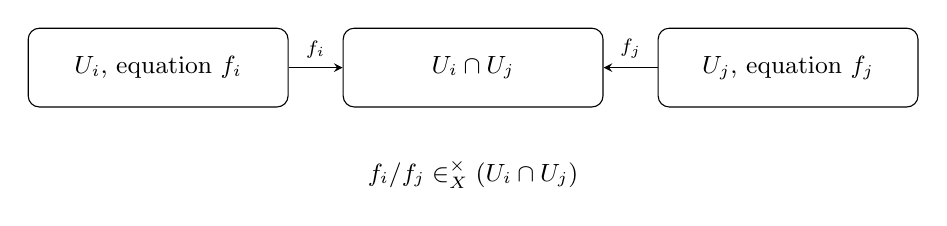
\begin{tikzpicture}[>=stealth,every node/.style={font=\small}]
\node[draw,rounded corners,minimum width=3.3cm,minimum height=1cm] (ui) at (-4,0) {$U_i$, equation $f_i$};
\node[draw,rounded corners,minimum width=3.3cm,minimum height=1cm] (ov) at (0,0) {$U_i\cap U_j$};
\node[draw,rounded corners,minimum width=3.3cm,minimum height=1cm] (uj) at (4,0) {$U_j$, equation $f_j$};
\draw[->] (ui)--node[above,font=\scriptsize]{$f_i$}(ov);
\draw[<-] (ov)--node[above,font=\scriptsize]{$f_j$}(uj);
\node at (0,-1.35) {$f_i/f_j\in\OO_X^\times(U_i\cap U_j)$};
\end{tikzpicture}
\caption{Local Cartier equations agree only up to a regular unit on overlaps.}
\label{fig:vi40-local-equations}
\end{figure}
